


\begin{document}
Three different op amp topologies were provided as part of the lab. The chosen circuit can be seen in can be seen in Figure \ref{fig:default}.

\begin{figure}[H]
    \begin{center}
    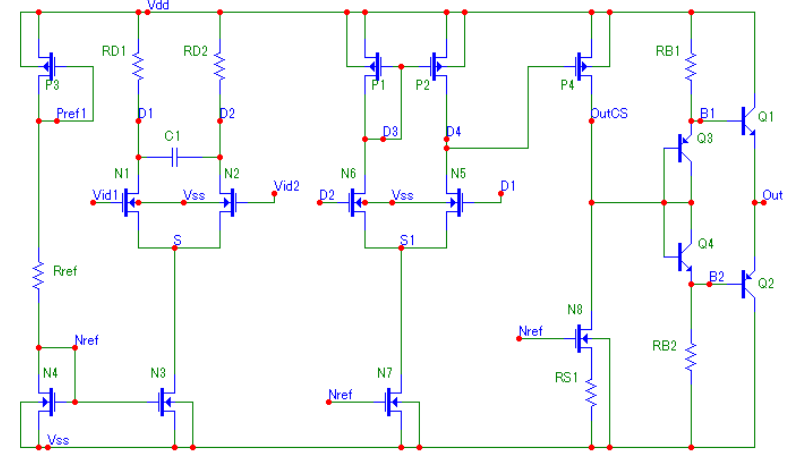
\includegraphics[scale=.45]{Simulations/default_circ.png}
    \caption{Generic schematic for chosen topology \cite{b2}}
    \label{fig:default}
    \end{center}
\end{figure}
This design was chosen due to the fact that every stage, with the exclusion of the output stage, was designed as part of lab 2 and 3. The stages can be broken down as such: a simple current mirror, a resistively loaded differential pair, an active loaded differential pair, an active load common source amplifier and finally a BJT amplifier output stage. The final simulated circuit can be seen in Figure \ref{fig:simcircuit}.

\begin{figure}[H]
    \begin{center}
    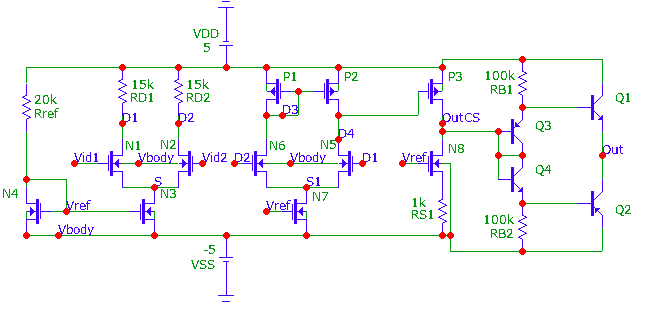
\includegraphics[scale=.55]{Simulations/simcircuit.png}
    \caption{Simulated op amp circuit}
    \label{fig:simcircuit}
    \end{center}
\end{figure}

The circuits will be simulated in MicroCap 11. The values for the components will initially be the values calculated in circuit development. The generic bias conditions for the ALD1106 and 1107 are summarized in Table \ref{tab:bias}. 

\begin{figure}[H]
	\begin{center}
		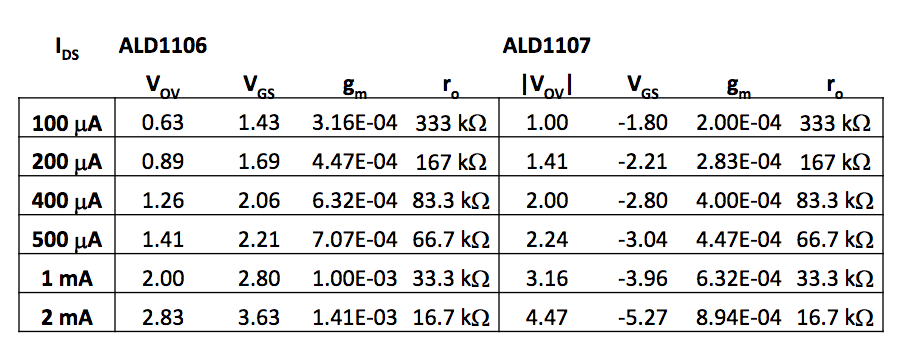
\includegraphics[scale=.35]{Simulations/nuribias.png}
		\caption{Typical ALD bias conditions \cite{b3}}
		\label{tab:bias}
	\end{center}
\end{figure}

Here the typical bias conditions for the constraining MOSFETs can be seen. For the purposes of this lab, the bias current of 400 $\mu$A was chosen.

\subsection{Resistively Loaded Differential Amplifier}

The resistively loaded amplifier stage requires a current mirror in order to generate the chosen bias current of 400 $\mu$A. This was achieved by applying Ohm's Law. The  V$_{gs}$ of the simple current mirror needs to be -3V. In order to  have the correct  current R$_{ref}$ was set to 20k$\Omega$. The simulated resistive load differential pair can be seen in Figure \ref{fig:ResLoadSim}.
\begin{figure}[H]
    \begin{center}
    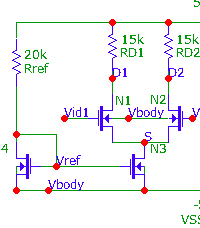
\includegraphics[scale=.85]{Simulations/simdiff.png}
    \caption{Simulated resistive load differential amplifier}
    \label{fig:ResLoadSim}
    \end{center}
\end{figure}

In addition, the current through the load resistors needs to be half of the bias current. As a result, the resistance values can be found by applying KVL which can be seen in Equation \ref{eqn:drainresist} 

\begin{equation}
V_{o_1} = V_{DD} - \frac{1}{2}I_{bias} R_d,
\label{eqn:drainresist}
\end{equation}

where V$_{DD}$ is the supply voltage. This leads to R$_{drain}$ of 15k$\Omega$.  The differential gain of the circuit can be found by Equation \ref{eq:Adsimresist} 
\begin{equation}\label{eq:Adsimresist}
A_d = g_m R_d,
\end{equation}

where g$_m$ is the transconductance of the amplifying NMOS and R$_d$ is the drain resistance and was calculated to be 16 dB. The output is double ended due to it feeding another amplifier stage. The simulated gain can be seen in  Figure \ref{fig:adsimresist}.


\begin{figure}[H]
    \begin{center}
    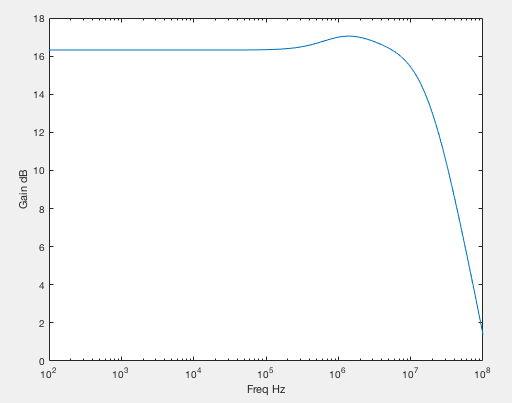
\includegraphics[scale=.30]{Simulations/gainfirststage.png}
    \caption{Simulated resistive load differential gain}
    \label{fig:adsimresist}
    \end{center}
\end{figure}
This was measured by performing an AC analysis in Microcap from 100Hz to 1MHz. This was performed by grounding one of the inputs whilest measuring the voltage differentially from the output nodes. The simulated value was marginally higher at 16.2 dB. The simulated phase can be seen in Figure  \ref{fig:firststagephase}.

\begin{figure}[H]
	\begin{center}
		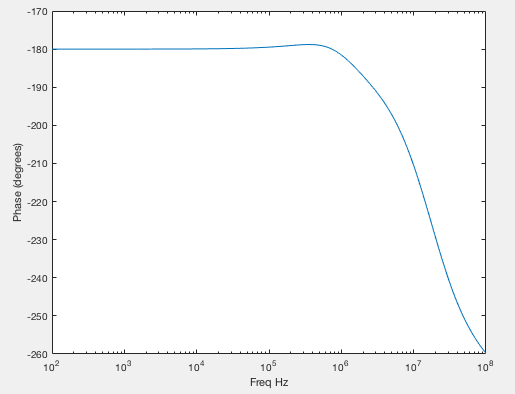
\includegraphics[scale=.30]{Simulations/phasefirststage.png}
		\caption{Simulated resistive load differential phase}
		\label{fig:firststagephase}.
	\end{center}
\end{figure}

The phase can be seen to be 180 degrees stable until 1 MHz. This is desirable for an input stage, which is why the differential pair was chosen as the first stage. This stage was then cascaded with an active load differential pair.


\subsection{Active Load Differential Pair}
The next stage of op amp is the active load differential pair. This circuit is identical to that designed in Task 3.  This circuit can be seen in Figure \ref{fig:ActiveLoadSim}. This modification allows for the single ended output to achieve gain that is comparable to that of the active load with a double ended output.


\begin{figure}[H]
    \begin{center}
    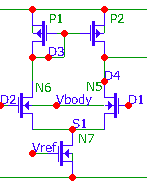
\includegraphics[scale=.85]{Simulations/simactive.png}
    \caption{Simulated active load differential amplifier}
    \label{fig:ActiveLoadSim}
    \end{center}
\end{figure}

The differential gain for an actively loaded differential pair can be seen with Equation \ref{eq:Adsimactive}
\begin{equation}
A_d = g_{m_N}(r_{o_P}||r_{o_N}),
\label{eqn:Ad_Active_Load}
\end{equation}

where  r$_o$ is the small signal output resistance of a MOSFET which is found by the Equation \ref{eq:ro}

\begin{equation}
r_o = \frac{1}{\lambda I_{DS}},
\label{eqn:ro}
\end{equation}

where  $\lambda$ is the channel length modulation parameter. The output resistance for NMOS is found to be 172k$\Omega$ and PMOS is found to be 162k$\Omega$. he differential gain was calculated to be 35 dB. The simulated differential gain for the active load can be seen in Figure \ref{fig:activeAdsim}.


\begin{figure}[H]
    \begin{center}
    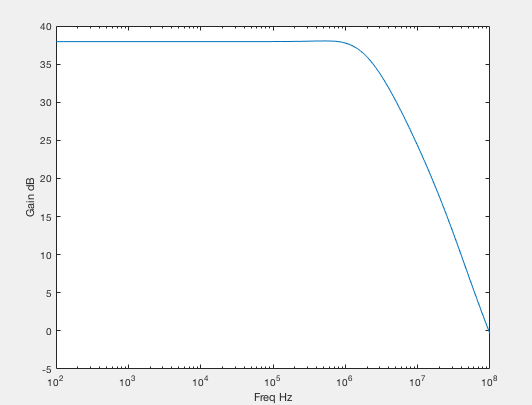
\includegraphics[scale=.30]{Simulations/gainsecondstage.png}
    \caption{Simulated active load differential gain}
    \label{fig:activeAdsim}
    \end{center}
\end{figure}

This simulation was performed in the same manner as the resistive load. The differential gain is found to be much high than resistive load at 38 dB and consistent with the calculated value of 35 dB. The phase of the active load can be seen in Figure \ref{fig:activephase}.
\begin{figure}[H]
	\begin{center}
		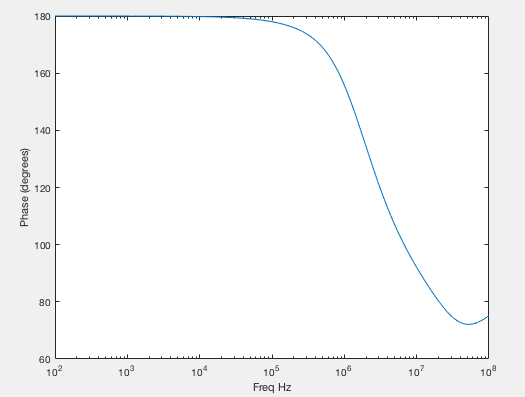
\includegraphics[scale=.30]{Simulations/phase_secondstage.png}
		\caption{Simulated active load differential phase}
		\label{fig:activephase}
	\end{center}
\end{figure}
This stage can be seen to only be 180 degree stable until 100 kHz. This is the minimum required by the lab specifications. This stage is then passed to an active loaded common source stage.

\subsection{Common Source Amplifier}

The common source amplifier features an active load which serves as a biasing network. The common source allows for the output loading effects of the active load to be ignored due to the near infinite input impedence seen at the gate of the common source. The simulated circuit can be seen in Figure \ref{fig:simcs}.

\begin{figure}[H]
	\begin{center}
		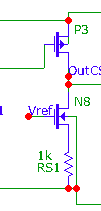
\includegraphics[scale=.65]{Simulations/simcs.png}
		\caption{Simulated common source amplifier}
		\label{fig:simcs}
	\end{center}
\end{figure} 

The voltage gain of a common source amplifier can be expressed in Equation \ref{eqn:csgain}


\begin{equation}
A_{vo} = -\frac{g_mR_d}{1+g_mR_s},
\label{eqn:csgain}
\end{equation}

where R$_s$ is the resistance seen at the source of the amplfying transistor which in this case is the r$_o$ of the active load. The gain can be calculated to be 23 dB. The active load features source degeneration, this resistor value should be large enough to ensure that with grounded inputs the common source output node is 0V. The resistor that achieved this is 1 k$\Omega$. The simulated gain can be seen in Figure \ref{fig:gaincs}.

\begin{figure}[H]
	\begin{center}
		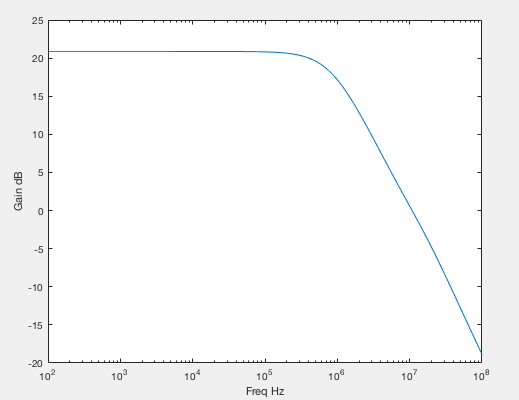
\includegraphics[scale=.40]{Simulations/gaincommonsource.png}
		\caption{Simulated common source amplifier gain}
		\label{fig:gaincs}
	\end{center}
\end{figure} 

The gain is slightly less than the calculated 23 dB at 20.5 dB. The phase the common source stage can be seen in Figure \ref{fig:csphase}.

\begin{figure}[H]
	\begin{center}
		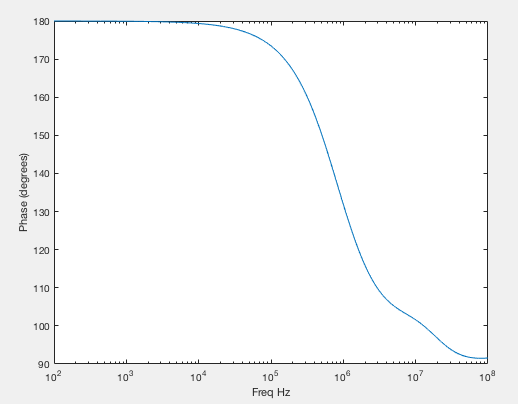
\includegraphics[scale=.40]{Simulations/phasecommonsource.png}
		\caption{Simulated common source amplifier phase}
		\label{fig:csphase}
	\end{center}
\end{figure} 

The common source, similar to that of the active load, is 180 degree stable until 100 kHz.  The common source is then fed to an output stage. The output stage will be covered in more detail in a later task. For the purposes of this lab the output stage can be treated as an emitter follower.

\subsection{Output Stage}

Due to the design of this stage being mostly beyond the scope of this task; the largest design consideration was choosing resistors values great enough to ensure that the base emitter voltages of remain less than 0.7V. These values were changed in Microcap until the correct bias conditions were found. The resistor values were found to be 100 k$\Omega$. The output gain can be expressed through Equation \ref{eq:efollower}

\begin{equation}
A_{vo} = \frac{g_mR_E}{g_mR_E + 1},
\label{eq:efollower}
\end{equation}

where R$_E$ is the resistance seen at the emitter of the BJT and g$_m$ is the transconductance on the  BJT. The gain can be calculated to be 0.96 V/V. The simulated gain can be seen in Figure \ref{fig:outputgain}.

\begin{figure}[H]
	\begin{center}
		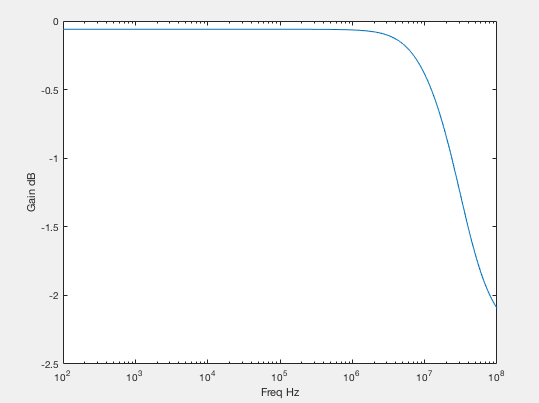
\includegraphics[scale=.40]{Simulations/gainlaststage.png}
		\caption{Simulated output stage gain}
		\label{fig:outputgain}
	\end{center}
\end{figure} 

The gain can be seen to be a little less than one, this is expected by the emitter follower nature of the stage. The Ideal emitter follower has a voltage gain of 1 V/V. The simulated phase can be seen in Figure \ref{fig:outputphase}.

\begin{figure}[H]
	\begin{center}
		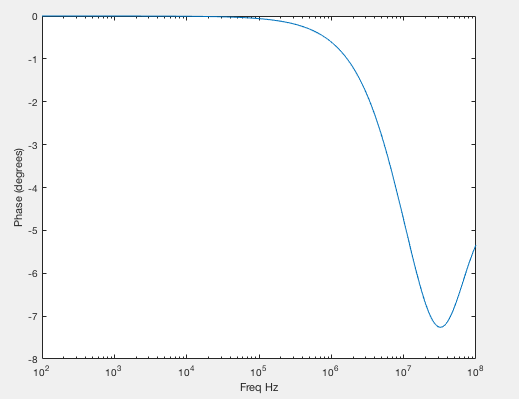
\includegraphics[scale=.40]{Simulations/phaselaststage.png}
		\caption{Simulated output stage phase}
		\label{fig:outputphase}
	\end{center}
\end{figure} 

The output stage remains 180 degree stable until 1 MHz, which is a decade higher than the previous two stages. The overall gain of the circuit can be seen in Figure \ref{fig:overallgain}. 

\begin{figure}[H]
	\begin{center}
		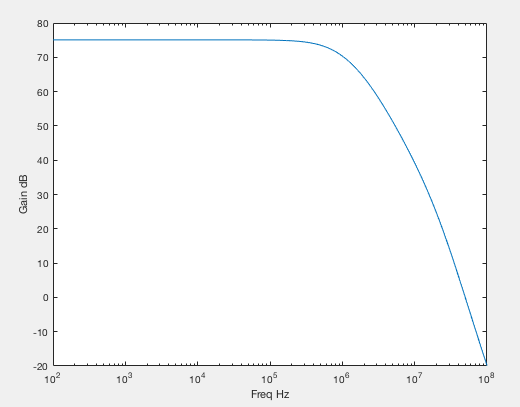
\includegraphics[scale=.40]{Simulations/gain_overall.png}
		\caption{Simulated overall gain}
		\label{fig:overallgain}
	\end{center}
\end{figure} 

The gain can be seen to be much greater than the required 46 dB at 75 dB. Care is necessary when building this circuit as very little input could result in a railed output. The final phase can be seen in Figure \ref{fig:overallphase}.


\begin{figure}[H]
	\begin{center}
		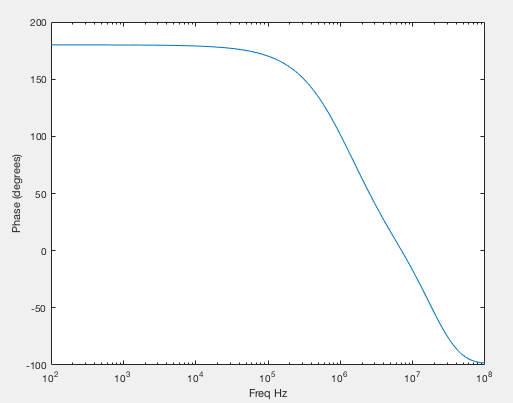
\includegraphics[scale=.40]{Simulations/phaseoverall.png}
		\caption{Simulated overall phase}
		\label{fig:overallphase}
	\end{center}
\end{figure} 

The final output can be seen to be 180 degree stable until 100 kHz, which is required by the specifications.
The DC bias conditions measured in Microcap can be seen in Table \ref{tab:simdcbias}.


\begin{table}[H]
	\centering
	\caption{DC bias values}
	\label{tab:simdcbias}
	\begin{tabular}{|l|l|}
		\hline
		\textbf{Simulated Values} &         \\ \hline
		Vref                        & -3.003V \\ \hline
		D1                          & 1.284V  \\ \hline
		D2                          & 1.284V  \\ \hline
		D3                          & 2.78V   \\ \hline
		D4                          & 2.78V   \\ \hline
		S                           & .972V   \\ \hline
		S1                          & -1.34V  \\ \hline
		OutCS                       & -82mV   \\ \hline
		Out                         & -11.4mV \\ \hline
		A$_d$ First Stage   &  16.2 dB \\ \hline
		A$_d$ Second Stage & 38 dB \\ \hline
		A$_{vo}$ Common source & 20.5 dB \\ \hline
		A$_{vo}$ Output Stage & -.1 dB \\ \hline
		A$_d$     Final &  75dB \\ \hline
	\end{tabular}
\end{table}

The DC bias conditions match that of this found in previous tasks. Notably the output of both the CS  and final stage is not 0V. This is due to body effect and channel length modulation effects, this voltage is known as the offset voltage.



\end{document}